\chapter{Structure \& Layout of Site}
Converting a youth campsite into a site for a youth camp is actually relatively simple. Biblins is a well equipped site in terms of water and waste disposal. Biblins not being on the mains electricity grid provided some challenges - which will be discussed in the Site Services section of this document, as well as the necessity for the use of bottled gas.\\

The decisions around how we use the different areas on site were taken over a number of months, involving different people at different times. The first decisions to be made were around how we would divide up the site. With the redevelopment work taking place in early 2023, the decisions around this were almost made for us: using pitches 1 through 3b as villages, pitches 4 and 5 for the central area and site services and pitches 5 through 11 as villages. This structure worked out very well in the end, as pitches 4 and 5 are the right size and location for central amenities for the camp.\\

The conversion of camping pitches to villages was slightly more challenging however. This was due to not knowing the size of villages until very late and even after having completed the village allocation process - it was difficult to visualise the size of a village. The first draft of site layout was completed by the Camp Coordinator and Chief Executive. This draft was circulated to those booked, which on discovering that the allocated pitches weren't what they seemed - was regarded as an error. The erroneous publication of pitches fell to human error when neither the camp coordinator nor the chief executive knew the sizes of pitches. The solution was found very quickly during On-Site Pre-Camp where a walk of the site was conducted and pitch sizes were re-allocated.

\begin{table}[ht]
    \centering
    {\RaggedRight
    \begin{tabular}{p{0.3\textwidth} p{0.6\textwidth}}
    \textbf{Pitches} & \textbf{Use}\\
    \hline
    \hline
    1a - 2a & Asgard Village (approx 90 campers) \\
    \hline
    2a - 3b & Benben village (approx 80 campers) \\
    \hline
    4 - 5 & Central Area \\
    \hline
    6 - 7a & Camelot Village (approx 90 campers) \\
    \hline
    7b - 8a & Dinas Affaraon Village (approx 90 campers) \\
    \hline
    8b - 11 & Elysium Village (approx 90 campers)\\
    \hline
    \end{tabular}
    } % end of rr     
    \caption{Use of pitches}
\end{table}

\begin{figure}[ht]
    \centering
    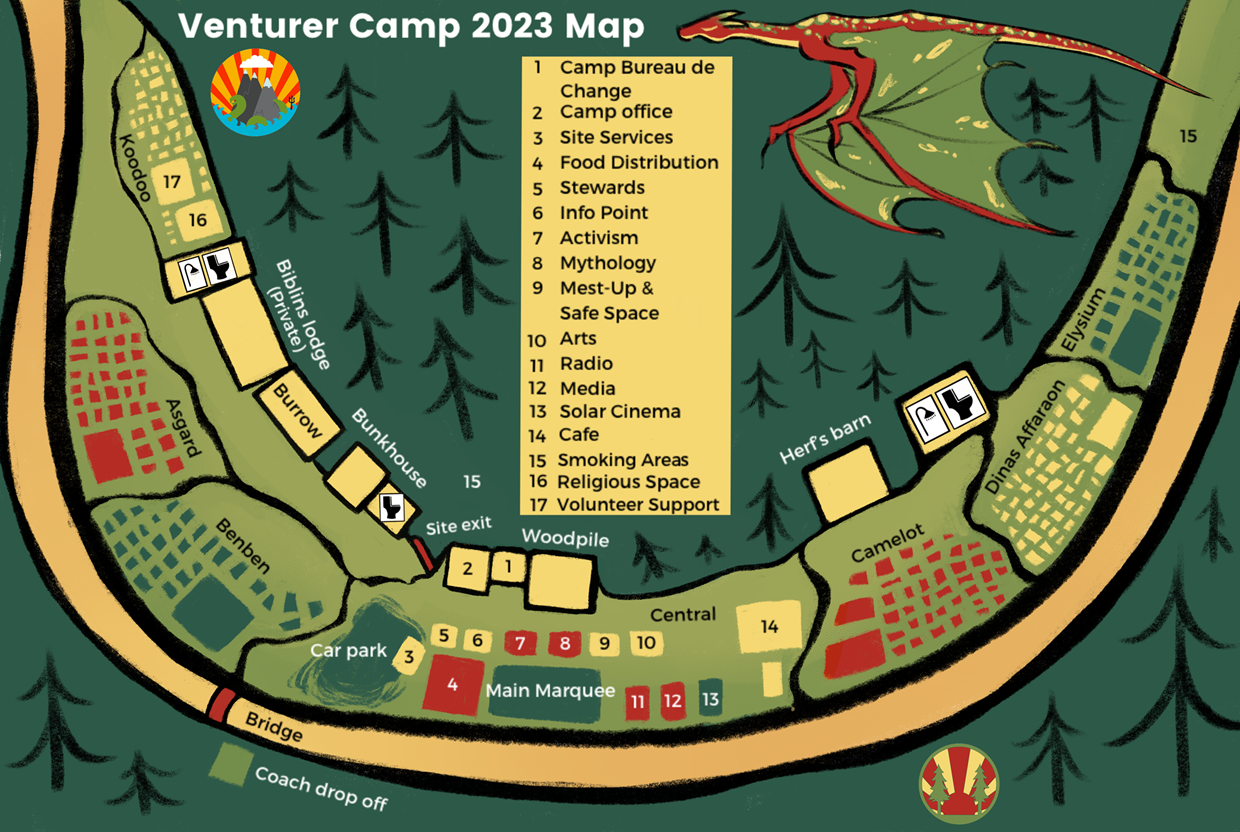
\includegraphics[width=0.8\textwidth]{assets/camp-map.png}
    \caption{Camp Map}
\end{figure}

\section{Village Pitch Allocation Feedback}
Generally, villages were content with their pitch allocations, other than two exceptions at either end of the site.\\

Due to ongoing waste water issues at the west-end of Biblins, the grey water septic tank was filling rapidly, causing it to overflow only days after it had been emptied. Before camp started, the Biblins staff team expanded the exclusion zone around the leaking drain cover and village adults were instructed to set up their village such that any food would be prepared as far away from `the spill' as possible. The overflowing water was regularly being tested by the local health authority, and the tests were coming back that the water was grey water not sewage, thus safe to let people near.
Due to the size of Asgard, the village adults took the decision to split their village into two, with a small group of people camping one side of the spill and the rest of their village situated on the other side. During the camp, a young person contacted home and mentioned that they were camping near `sewage'. This resulted in the exclusion zone around the leaking drain cover to be expanded, splitting Asgard in two, where previously there had been a small walkway and space for tents on the river-side of the spill, as far away from the drain cover as possible. Throughout the event, the Biblins staff team were monitoring the situation and the tank was pumped out twice. \\

At the other end of the site, Elysium was situated on a series of long and thin pitches. Thus resulting in their entire village being stretched out over a long distance. This meant that some members of the village were a substantial distance away from the village services (kitchen \& marquee), which had been situated as close to the Dinas Affaraon boundary as possible due to not having a tap closer than the Eastern toilet block. Due to the mish-mash composition of villages, given the low number of delegates from each group, Elysium turned into a collection of smaller circles of tents which some village residents found disjointing. A number of villages also found themselves in a similar situation with a few smaller circles of tents making up the village. 

\section{Central Team Placement}
recruiting someone to KP the central village - a decision was made to not have a central village. Difficulties in finding a location to have the central village came from initial plans involving using The Burrow, which was later promised to the Concordia volunteers. \\

The decision was taken to disperse the central team members through the five villages, into villages where they either had connections, or grouping teams together. This decision caused some apprehension within the team, especially around meals. This was due to historic events where the central team did not have food saved for them, resulting in them having to scrounge for scraps after volunteering over mealtimes to make the camp happen. These issues were circumvented at Venturer Camp - as extremely specific instructions were given to KPs through the Food team and through the Village Handbook. The Village Handbook also contained a list of those with central roles who had a legitimate need for food to either be held back or served at a strange time, to ensure a consistent message was communicated with the KPs. This system worked well for the most part.\\

It worked out that Camelot \& Benben housed the majority of the central team, this decision was made to reduce the commute of the central team. Villages worked very hard to accommodate these central team members, ensuring that they planned clans around the list of people who couldn't be relied on to be there. This worked very effectively at Venturer Camp 2023, however at larger events where the clan members are younger, less useful, or less-accustomed to Woodcrafts ways of working, then this may not have been as much of a success.

\section{Camp Office, Info Point \& Stewards HQ}
We took the decision to separate the Stewards HQ and Camp Office. This decision was taken to ensure that the camp admin team had a space where they could do administration without being interrupted by stewards! We decided to use the Cabin as the camp office, as this would ensure good internet connectivity and provide shelter from the elements and then use a marquee for the Stewards HQ.\\

The Camp Office resided in the ``living'' room of the cabin, with the option to use the bedrooms or garden for anything (for example, meetings) should they be required. The Biblins staff team worked out of the ``Office'' section of the cabin which worked well to a certain extent. While we aimed to be respectful of the staff in the office who needed to do their site related work, there were times where we were traipsing in and out of the cabin, through the office to our office talking to people. For incidents like this, it would have been preferred to have another space we could use for meetings. Therefore some meetings were conducted in the garden of the cabin, this gave greater space for larger meetings.\\

Stewards HQ was situated directly opposite the cabin. For the first day of camp - they also acted as the Sign In point, which worked very well as we were able to direct more complex sign in issues to the cabin while keeping a good flow of people signing in at the stewards HQ. \\

There was never really a defined ``go here first'' point, this caused some issues where people would gravitate towards the cabin to ask their questions, most commonly ``when will the bank be open'', where the answer could be given by the Stewards HQ / Info Point. For future events, it would be recommended to have a first line support who can escalate to the core camp team in the office where required. These two locations should ideally be close enough together to feel like a large team but independent enough that campers don't get confused. 
